    \subsection{Ambiente De Desarrollo}
    Durante el desarrollo de la presente librería se usó el sistema operativo MacOS, con la terminal que se incorpora por defecto en el mismo.
    El primer paso que se debe realizarse es colocarse en el directorio en el que se desea trabajar, esta librería se sitúa en la carpeta Documentos durante el desarrollo, usando el comando de la Figura 8.4 es posible cambiar de directorio, ejecutandolo en la terminal.
    
    \newline
     \begin{figure}[H]
     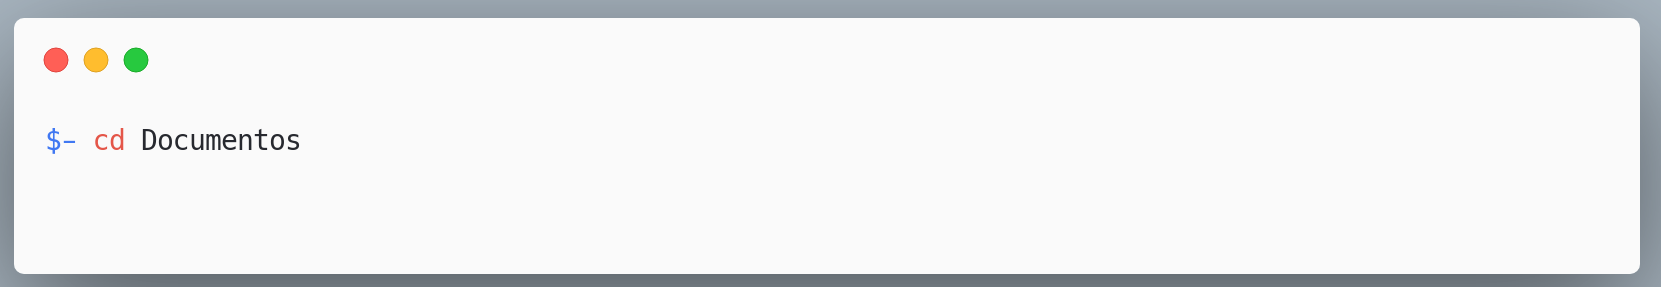
\includegraphics[width=1\textwidth]{./Imagenes/image15.png}
     \caption[Moverse entre directorios]{Moverse entre directorios}
         \end{figure}
Después se creó la carpeta de desarrollo son el siguente comando. Se llamó de manera simbólica como “crown”, que significa en español “corona”.
     \begin{figure}[H]
    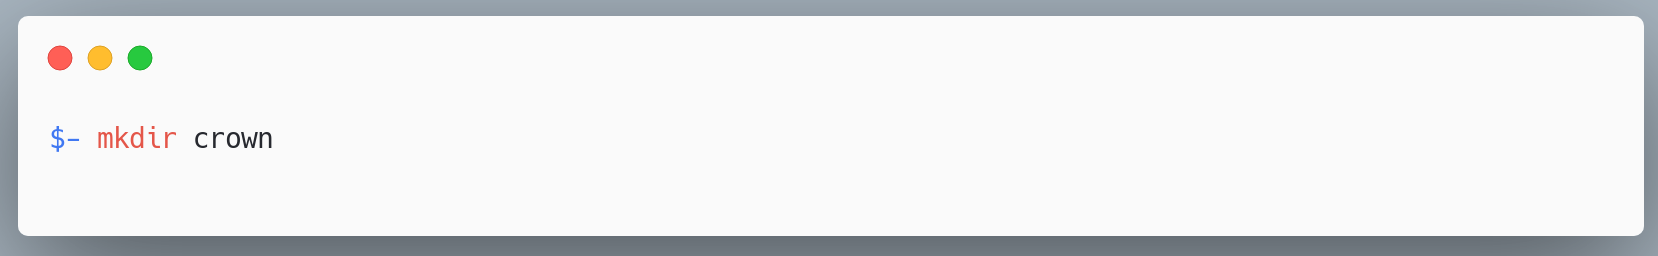
\includegraphics[width=1\textwidth]{./Imagenes/image7.png}
     \caption[Crear nuevo directorio]{Crear nuevo directorio}
         \end{figure}
    
    Dentro de esta carpeta debemos crear dos carpetas, una tendrá el código fuente, y la otra tendrá el resultado del código procesado que se importará por otros proyectos, con la ayuda del siguiente comando.
    \newline
     \begin{figure}[hbt!]
    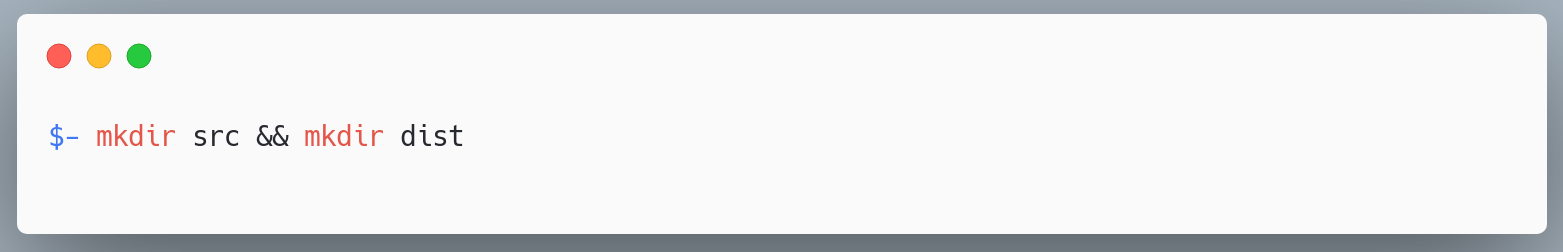
\includegraphics[width=1\textwidth]{./Imagenes/image37.png}
     \caption[Crear nuevos directorios]{Crear nuevos directorios}
         \end{figure}
    \newline
    \newline
    
    \subsection{Inicialización Del Archivo NPM}
    Se continúo inicializando el archivo de NPM, el cual nos sirve para llevar el control de las dependencias de JavaScript que se vayan agregando, esto ejecutando el siguiente comando.
    \newline
    \newline
     \begin{figure}[H]
    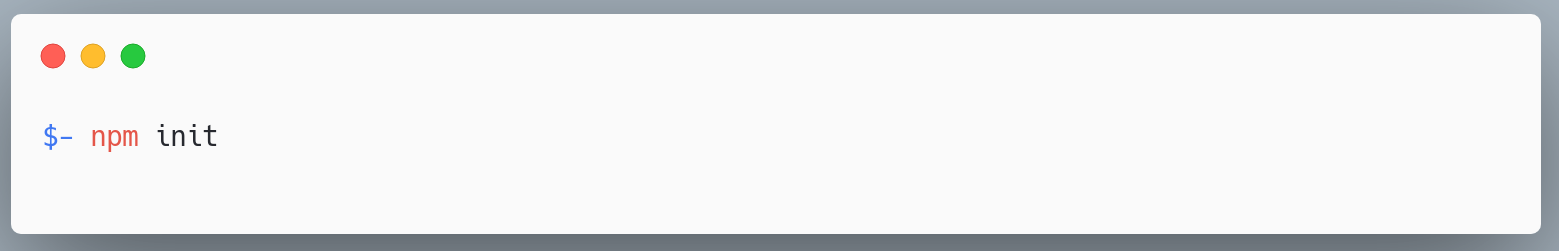
\includegraphics[width=1\textwidth]{./Imagenes/image11.png}
     \caption[Inicializar NPM]{Inicializar NPM}
         \end{figure}
    
    \newline
    \newline
    Al introducir el comando anterior este preguntara por una lista de datos necesarios, para tener el control de los paquetes, estos son los siguientes datos que se deben proporcionar:
    \begin{itemize}
    \item \textbf{Nombre del paquete:} Este es el nombre simbólico con el cual se puede identificar el paquete dentro del buscador de NPM, por lo tanto, es el nombre con el que nuestro paquete será encontrado.
    \item \textbf{Versión del paquete:}Con esta opción controlaremos la versión, y en caso de que se agreguen funcionalidades o se resuelva algún error, tendremos una manera de actualizar en los proyectos que incorporen esta librería.
    \item \textbf{Descripción del paquete: }Daremos a las personas una muy breve explicación acerca del uso que puedes obtener con nuestra librería.
    \item \textbf{Punto de entrada del paquete:} Es el directorio el cual será importado cuando agreguemos nuestra librería a otros proyectos, este podrá incluir la lógica o que solamente sea el nodo inicial de todo nuestro código.
    \item \textbf{Comando de prueba:} Dentro de este archivo nos permite incluir comandos que afectan a nuestra librería, en este caso, este comando nos sirve para ejecutar una serie de pruebas, para usar antes de publicar una nueva versión.
    \item \textbf{Repositorio de GIT del paquete:} Dentro de esta línea, debemos poner la dirección url en el cual está alojado nuestro proyecto. Este será agregado más adelante junto con el archivo de configuración de GIT.
    \item \textbf{Palabras clave del paquete:} Es una lista de palabras la cual nos ayuda para el momento cuando se inserta una búsqueda en el gestor de NPM, y pueda realizar una búsqueda basada en las palabras que describen la utilidad de nuestro paquete.
    \item \textbf{Autor del paquete:} Es el nombre del autor, autores u organización la cual está desarrollando el proyecto.
    \item \textbf{Licencia del paquete:} Existen una serie de licencias posibles a ser seleccionadas, para este caso se eligió la licencia MIT (MIT, Massachusetts Institute of Technology), que es una licencia de software que fue originada por el Instituto Tecnológico de Massachusetts, significa que el código que es producido bajo esta licencia es de uso libre, con la que damos muy pocas limitaciones de reutilización del código 
    \end{itemize}
    En la siguiente imagen se muestra un ejemplo de los datos solicitados por el comando y los datos introducidos, los cuales son de prueba y nos son los mismos que se ingresaron el proyecto original. 
    Todo esto generará un archivo final llamado package.json en el directorio raíz, este contendrá la configuración dada en este paso.
    Finalmente preguntará si la información introducida es correcta  y nos confirmara con una impresión en consola de los datos que estarán almacenados en el archivo.
    \newline
    \newline
     \begin{figure}[H]
    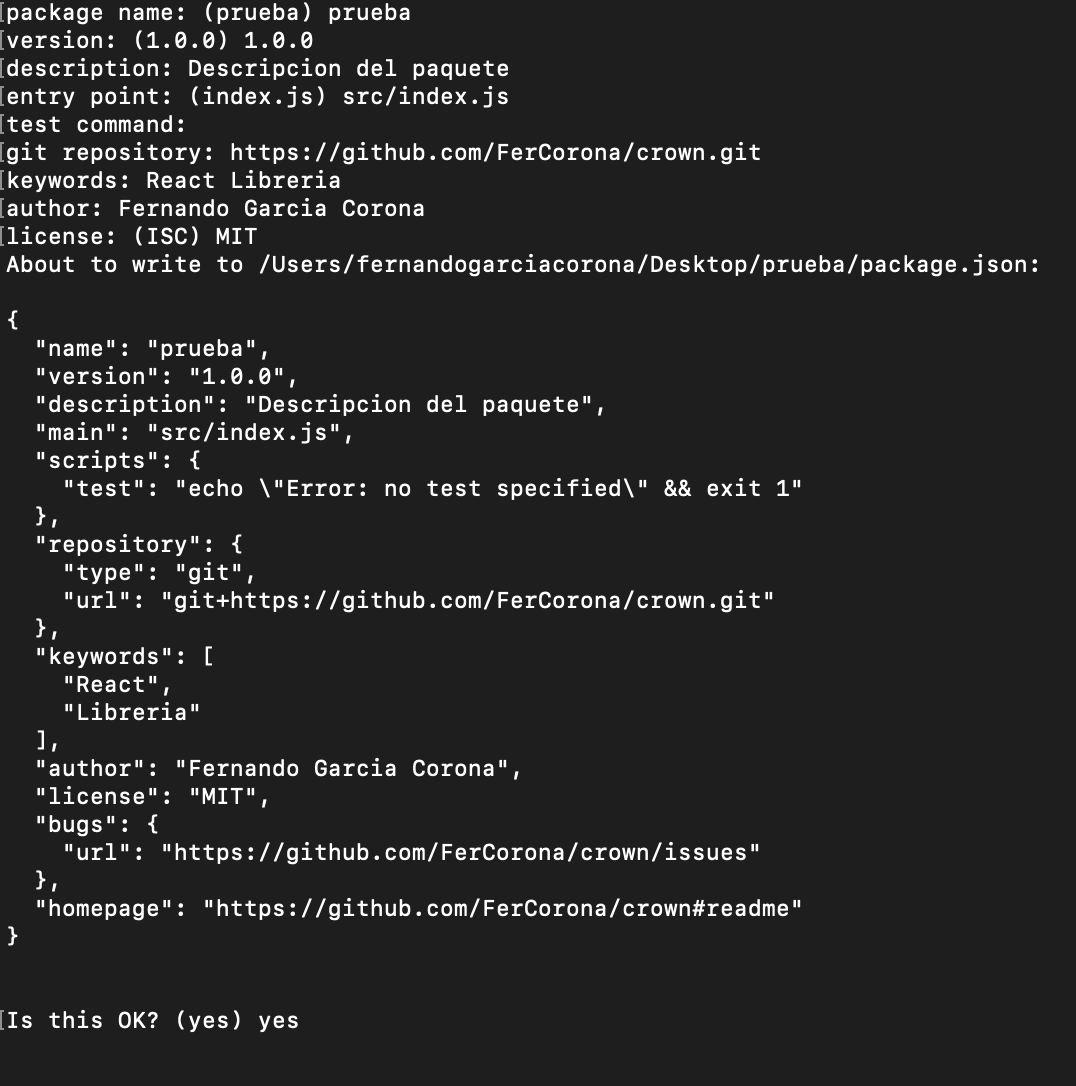
\includegraphics[width=1\textwidth]{./Imagenes/image9.png}
     \caption[Archivo de salida]{Archivo de salida}
         \end{figure}
    \newline
    \newline
    
    \subsection{Inicialización De Git En Nuestro Proyecto }
    Ahora se continuará agregando GIT en nuestro proyecto, esto nos garantizara el control de los cambios que se vayan realizando, para en caso de catástrofes poder regresar a una versión anterior, También podemos crear ramas,  para alojar nuevas funcionalidades que se requieran ser agregadas, eso sin afectar el estado del proyecto que ya está funcionando y cuando la nueva función esté completa y probada poder mezclarla con el original (la rama master).
    Incluir GIT no es una tarea compleja, basta con ejecutar el siguiente comando en la línea de comandos, esto dentro de nuestro directorio (“/Documents/crown”).
    \newline
    \newline
     \begin{figure}[H]
    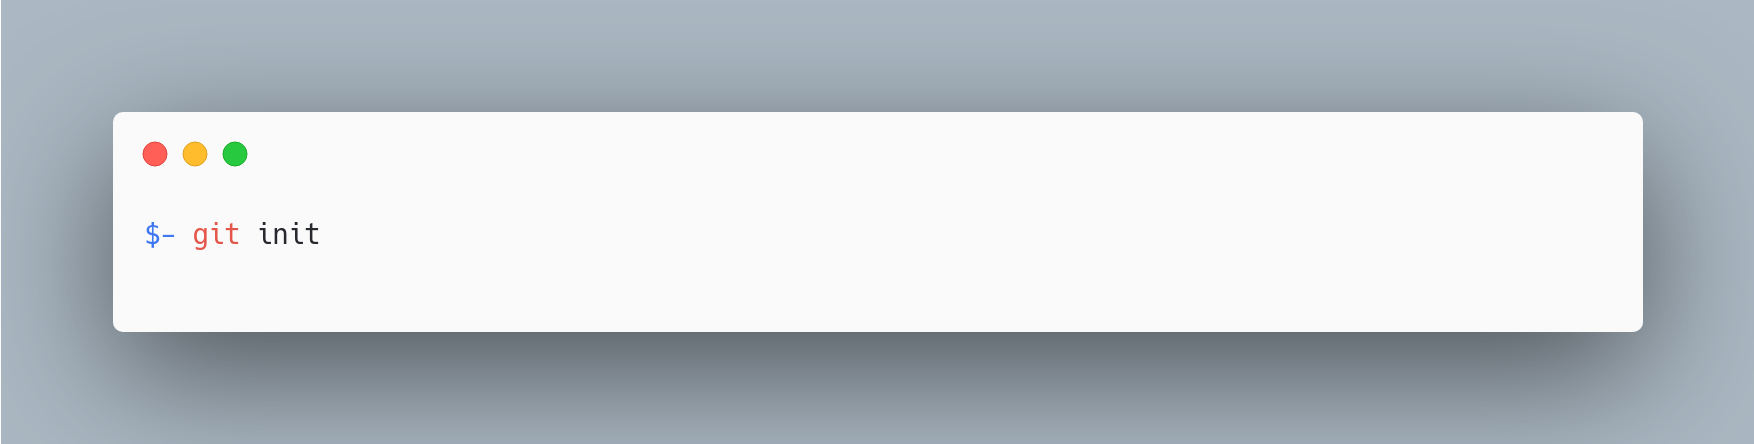
\includegraphics[width=1\textwidth]{./Imagenes/image35.png}
     \caption[Inicializar GIT]{Inicializar GIT}
         \end{figure}
    \newline
    \newline
    Creará una carpeta oculta (“/.git”) que nos permitirá manipular nuestro código con la línea de comandos de git, como crear ramas, hacer commit, hacer el merge de una rama etc.
    Para que esto funcione es necesario que el archivo creado anteriormente “package.json” conozca la ubicación remota de nuestro repositorio, se creó una cuenta en GITHUB  y se agregó un repositorio, el cual debemos copiar la dirección url y pegarla en el archivo “package.json”,  en el apartado llamado “repository” , en la llave “url” como se muestra en la imagen.
    Al la url que acabamos de copiar agregamos el prefijo “git+” y el postfijo “.git”.
    \newline
    \newline
     \begin{figure}[H]
    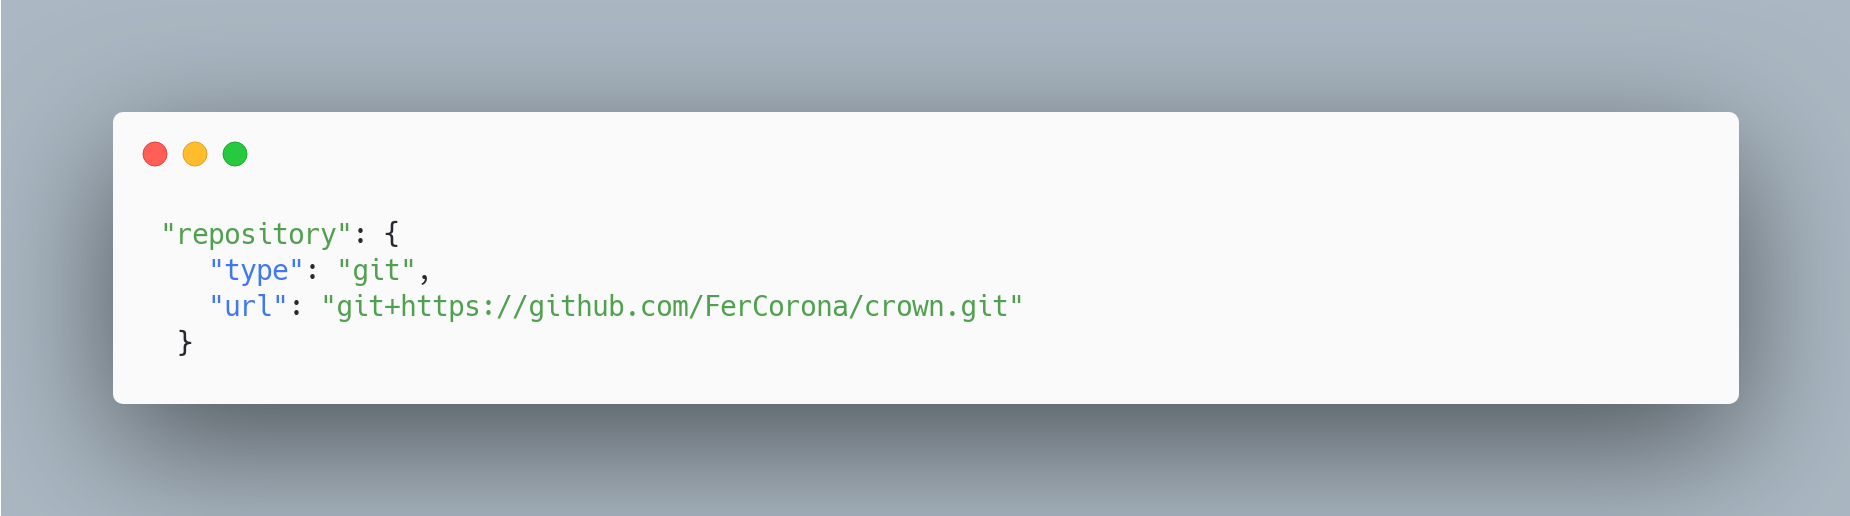
\includegraphics[width=1\textwidth]{./Imagenes/image4.png}
     \caption[Agregar repositorio existente]{Agregar repositorio existente}
         \end{figure}
    \newline
    \newline
    
    \subsection{Configuración Web-pack}
    Webpack es una tecnología utilizada en gran cantidad de proyectos de Front-end. Es útil cuando se trabaja en base a una estructura modular, en este caso modula nuestra librería para poder ser agregada en otros proyectos. Nos permite que el resultado final de nuestro proyecto sea menos pesado, esto es logrado por que concatena el código eliminando espacios no necesarios para el intérprete del navegador, lo que deja un archivo con código que no es del todo entendible para las personas pero que es muchos bits menos pesado para el navegador.
    También nos permite agregar cargadores para que pueda soportar SCSS, HTML JSX imágenes y otros archivos más.
    Para hacerlo funcionar debemos ejecutar una serie de comandos, que se enlistan a continuación, con ayuda de NPM.
    \newline
    \newline
     \begin{figure}[H]
    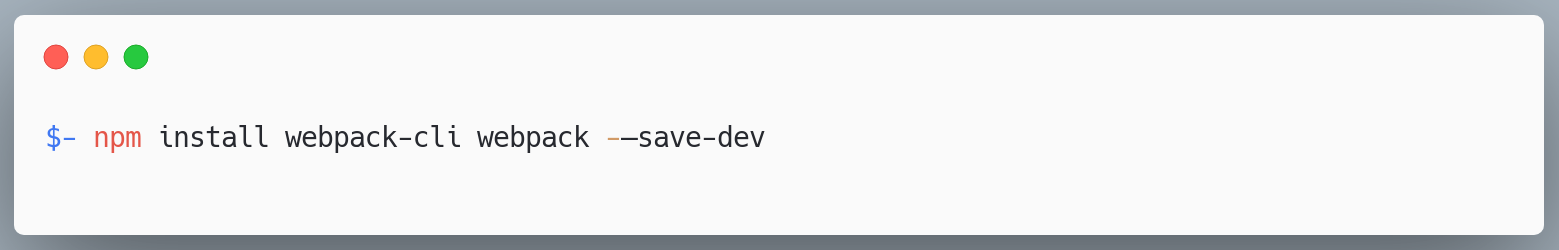
\includegraphics[width=1\textwidth]{./Imagenes/image3.png}
     \caption[Agregar Webpack]{Agregar Webpack}
         \end{figure}
    \newline
    \newline
    Los anteriores comandos agregan al proyecto en núcleo de Webpack, así como su cliente de comandos para la manipulación y visualización de archivos. Después de ejecutar los comandos se debe agregar los siguientes comandos en archivo “package.json”  en la sección de scripts, los script son los siguientes.
    \newline
    \newline
     \begin{figure}[H]
    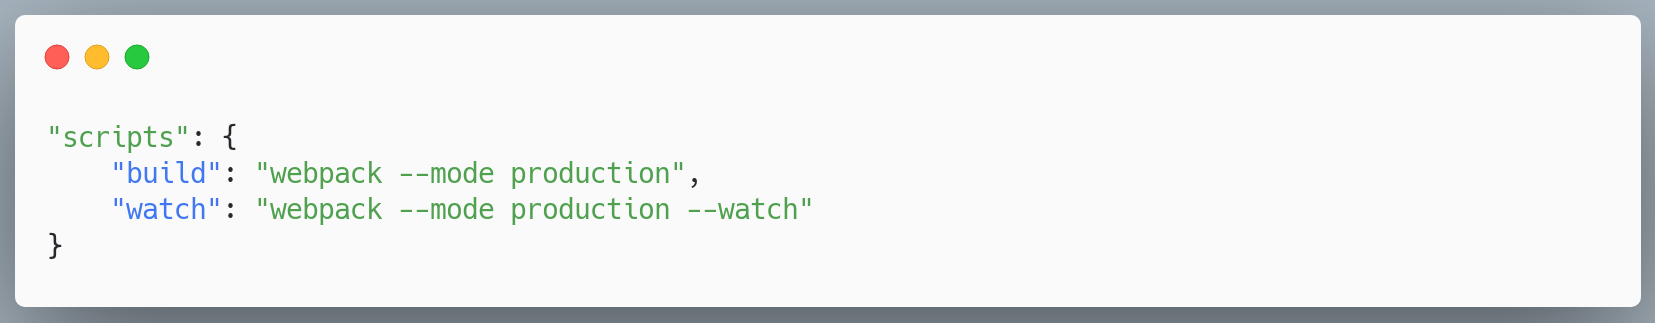
\includegraphics[width=1\textwidth]{./Imagenes/image6.png}
     \caption[Agregar scripts]{Agregar scripts}
         \end{figure}
    \newline
    \newline
    Los comandos agregados nos son de utilidad para:
    \begin{itemize}
    \item \textbf{Build:} Crear un archivo que estará listo para producción.
    \item \textbf{Watch:} Nos proporciona la misma funcionalidad que Build pero este, puede observar los cambios que estamos haciendo en tiempo real y actualizará el archivo final cada vez.
    \end{itemize}
    Para agregar configuración es necesario crear un archivo como se ilustra con el siguiente comando, estando en el directorio raíz de “crown”.
    \newline
    \newline
     \begin{figure}[H]
    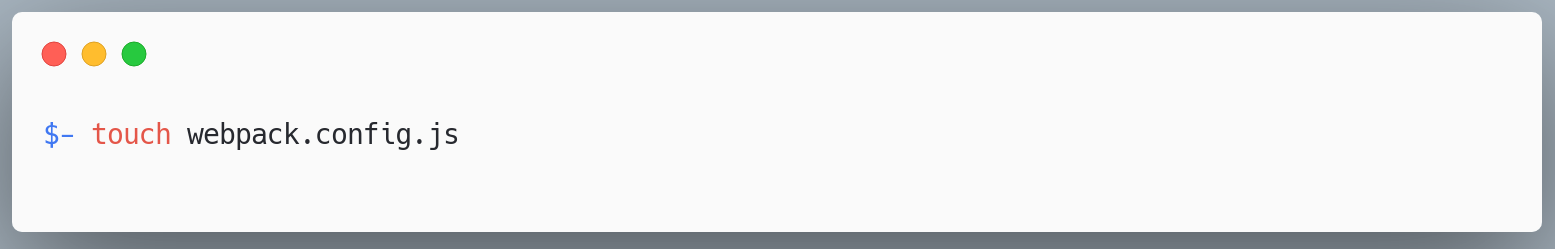
\includegraphics[width=1\textwidth]{./Imagenes/image38.png}
     \caption[Crear archivo vacío]{Crear archivo vacío}
         \end{figure}
    \newline
    Necesitamos agregar ciertos cargadores de WEPACK para poder usar SASS y CSS, con el siguiente comando.
    \newline
    \newline
     \begin{figure}[H]
    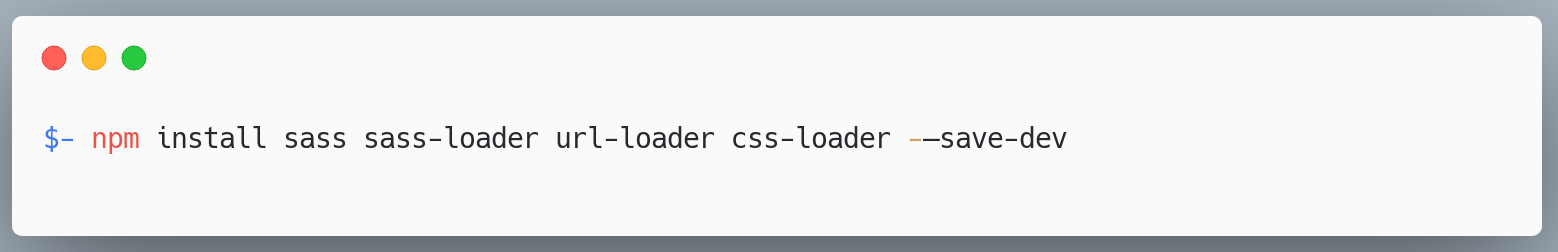
\includegraphics[width=1\textwidth]{./Imagenes/image8.png}
     \caption[Agregar cargadores de css]{Agregar cargadores de css}
         \end{figure}
    \newline
    \newline
    Con esto tenemos listas las dependencias necesarias para usar SASS / CSS y para poder manejar archivos como imágenes en JavaScript, tenemos que agregar la siguiente configuración en nuestro archivo Webpack.config.js.
    \newline
    \newline
     \begin{figure}[H]
    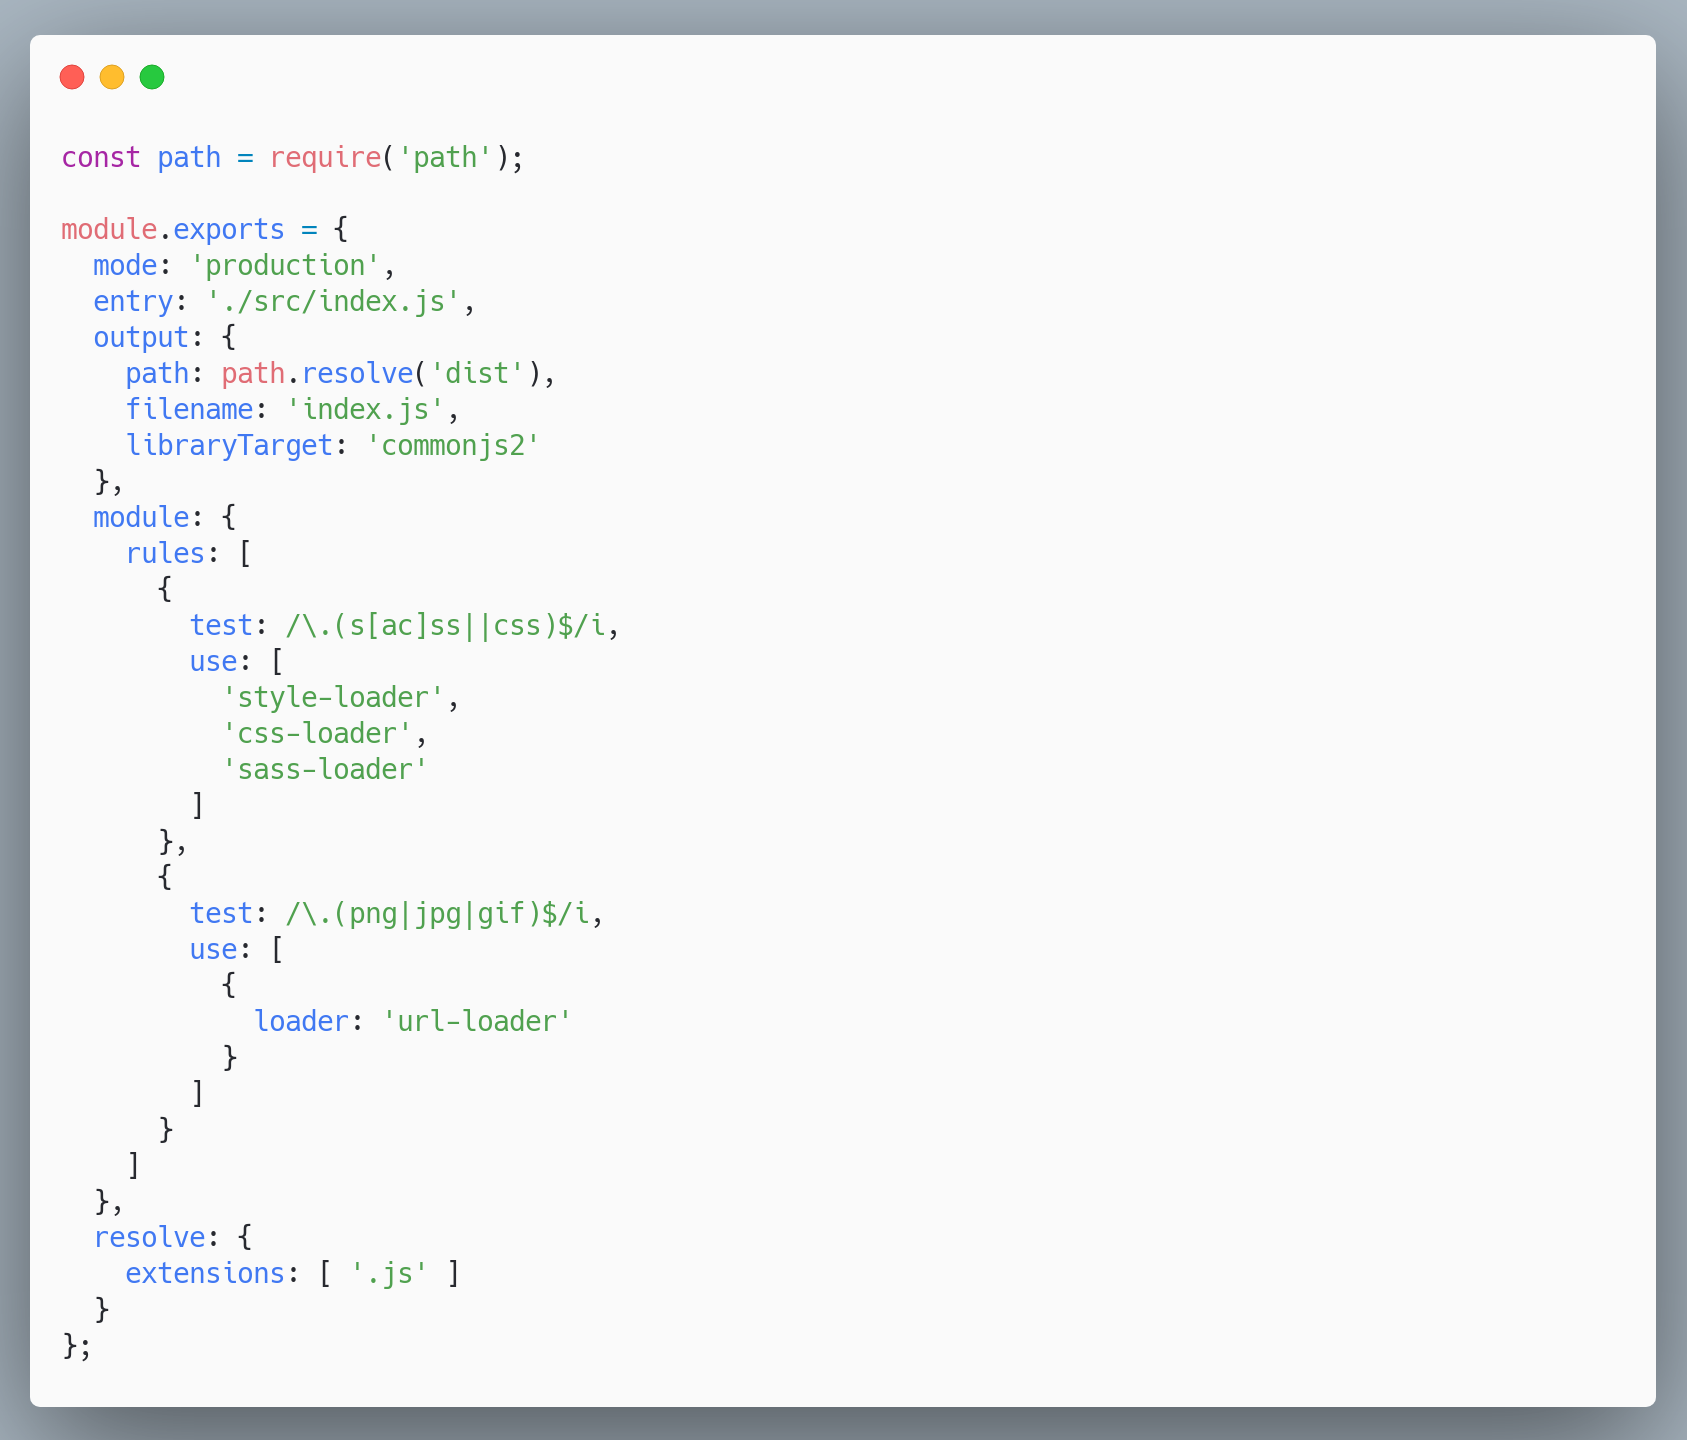
\includegraphics[width=1\textwidth]{./Imagenes/image2.png}
     \caption[Archivo final]{Archivo final}
         \end{figure}
    \newline
    La anterior configuración muestra cómo debe procesar cada tipo de archivo que encuentre dentro de nuestro proyecto, por eso dada una expresión regular que define extensiones de archivos puede usar un cargador a usar.
    Lo que es definido en la configuración es:
    \begin{itemize}
    \item \textbf{Entry: } Es el archivo inicial sobre el cual empezará el análisis del código si este tiene un import de otro archivo continuará sobre ese, esto generará un árbol. El directorio /src/index.js fue el dado para este caso.
    \item \textbf{Output: } Es el archivo en el que quedará la salida de nuestra librería en la dirección /dist/index.js
    \item \textbf{Rules: }Está incluido dentro de los módulos, esto agrega la manera en cómo se procesarán los archivos SCSS y CSS  con las dependencias style-loader, css-loader, sass-loader y por otra parte las imágenes con url-loader.
    \end{itemize}
    
    
    \subsection{Configuración Babel}
    Babel es un traductor de código JavaScript que permite convertir código de nuevas generaciones como el ES6 a versiones antiguas, extendiendo la compatibilidad a navegadores más viejos como Internet Explorer.
    Solo es necesario agregar las siguientes dependencias, con el siguiente comando.
    \newline
    \newline
     \begin{figure}[H]
    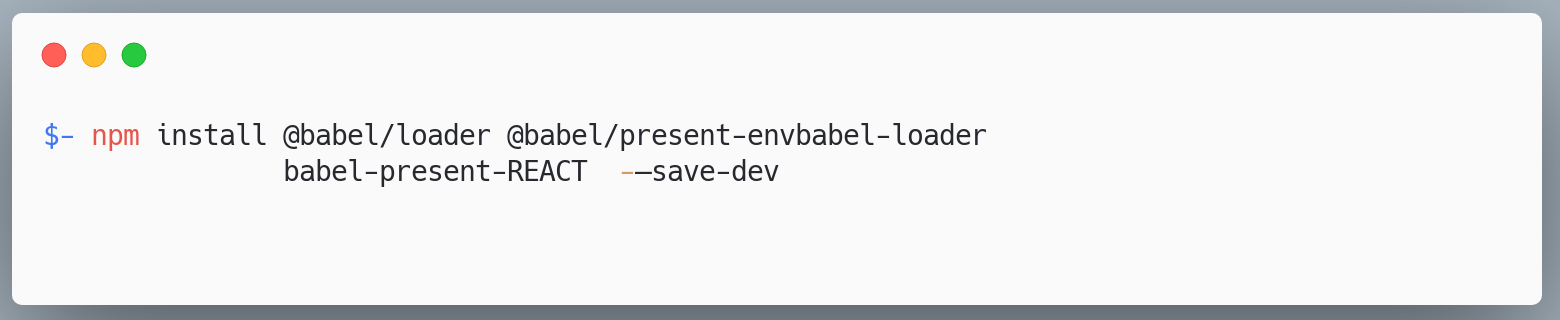
\includegraphics[width=1\textwidth]{./Imagenes/image36.png}
     \caption[Archivo Babel]{Archivo Babel}
         \end{figure}
    \newline
    \newline
    Después debemos crear un archivo en el directorio raíz llamado “.Babelrc”, al cual debemos agregar la siguiente configuración.
    \newline
    \newline
     \begin{figure}[H]
    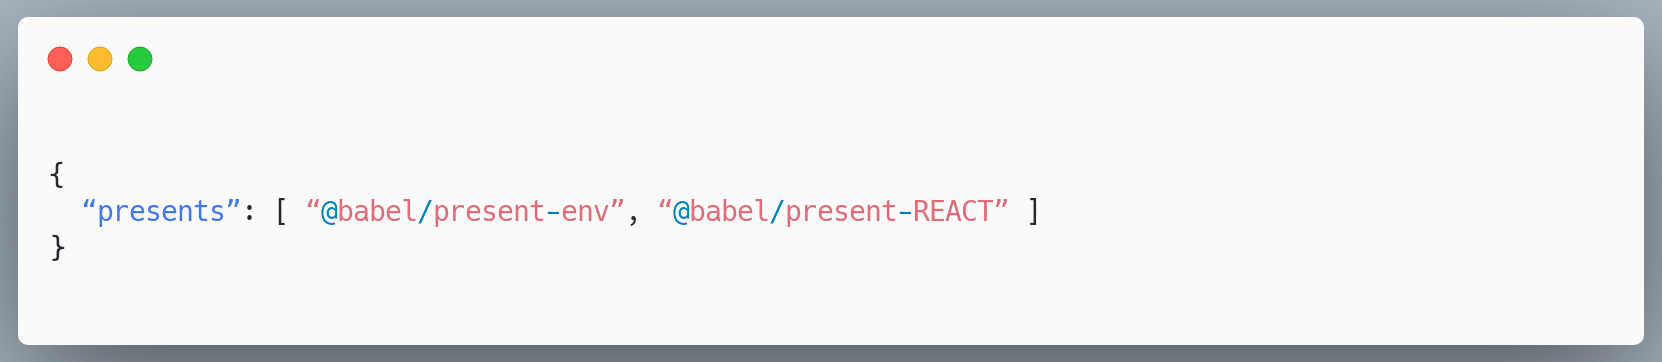
\includegraphics[width=1\textwidth]{./Imagenes/image17.png}
    \caption[Configurar Babel]{Configurar Babel}
    \end{figure}
    \newline
    \newline
    Y finalmente solo debemos agregar la siguiente configuración al archivo Webpack.config.js en el apartado de “rules” dentro de “module”.
    \newline
    \newline
     \begin{figure}[H]
    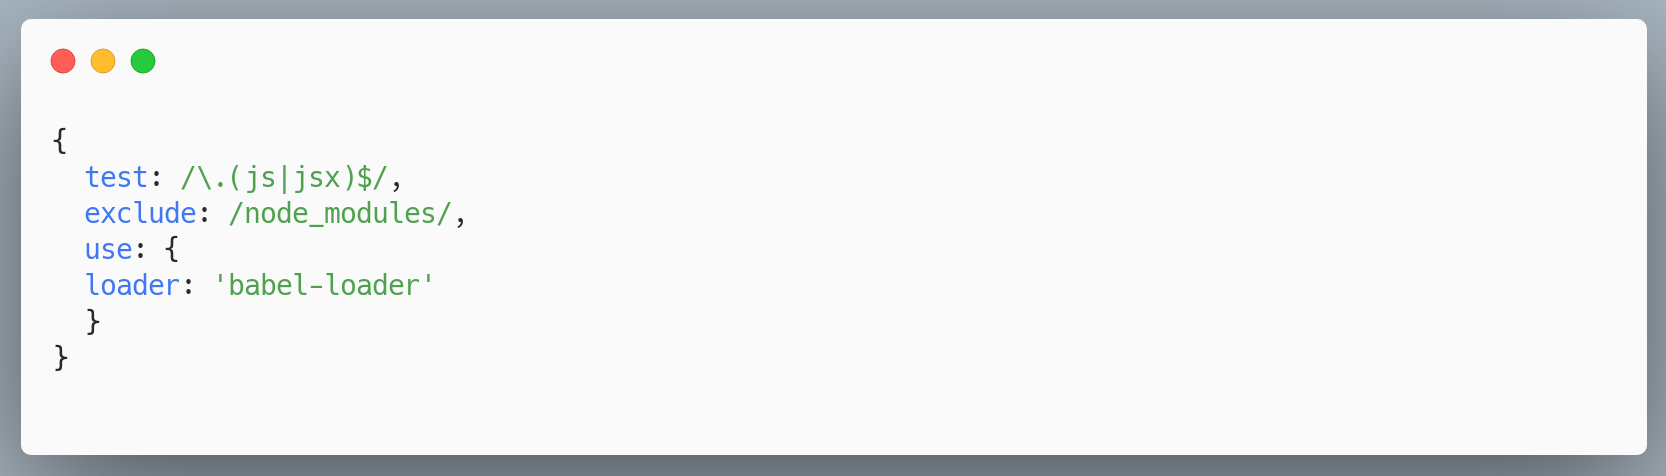
\includegraphics[width=1\textwidth]{./Imagenes/image1.png}
    \caption[Agregar Babel en Webpack]{Agregar Babel en Webpack}
    \end{figure}
    \newline
    \newline
    Esto para que WEWPACK sea el encargado de traducir el código con ayuda de Babel.
    
    
    \subsection{Agregar React Al Proyecto}
    React es una parte fundamental en el desarrollo de la presente librería y para agregarlo es necesario ejecutar el siguiente comando.
    \newline
    \newline
     \begin{figure}[H]
    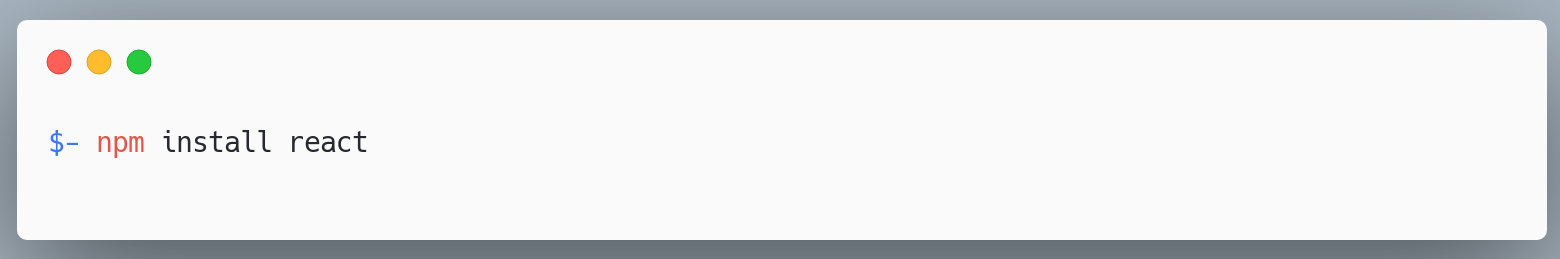
\includegraphics[width=1\textwidth]{./Imagenes/image23.png}
    \caption[Agregar React]{Agregar React}
    \end{figure}
    \newline
    \newline
    Para este comando no se agrega la bandera “–save-dev” al final, por que de esta manera forzamos a que cuando se instale esta librería también se instale React en caso de que no estuviera, ya que nuestra librería necesita React para su ejecución.
    
    
    \subsection{Configuración ESLint }
    Finalmente, para que nuestro espacio de desarrollo quede listo agregaremos ESLint que es un verificador de sintaxis, para tener un código limpio, con una clara indentación. Para que en toda la librería tengamos un código unificado. De igual manera no tendremos que preocuparnos por esto si no que al guardar el archivo obtenga el formato correcto.
    Para esto debemos ejecutar las siguientes dependencias en la terminal.
    \newline
    \newline
     \begin{figure}[H]
    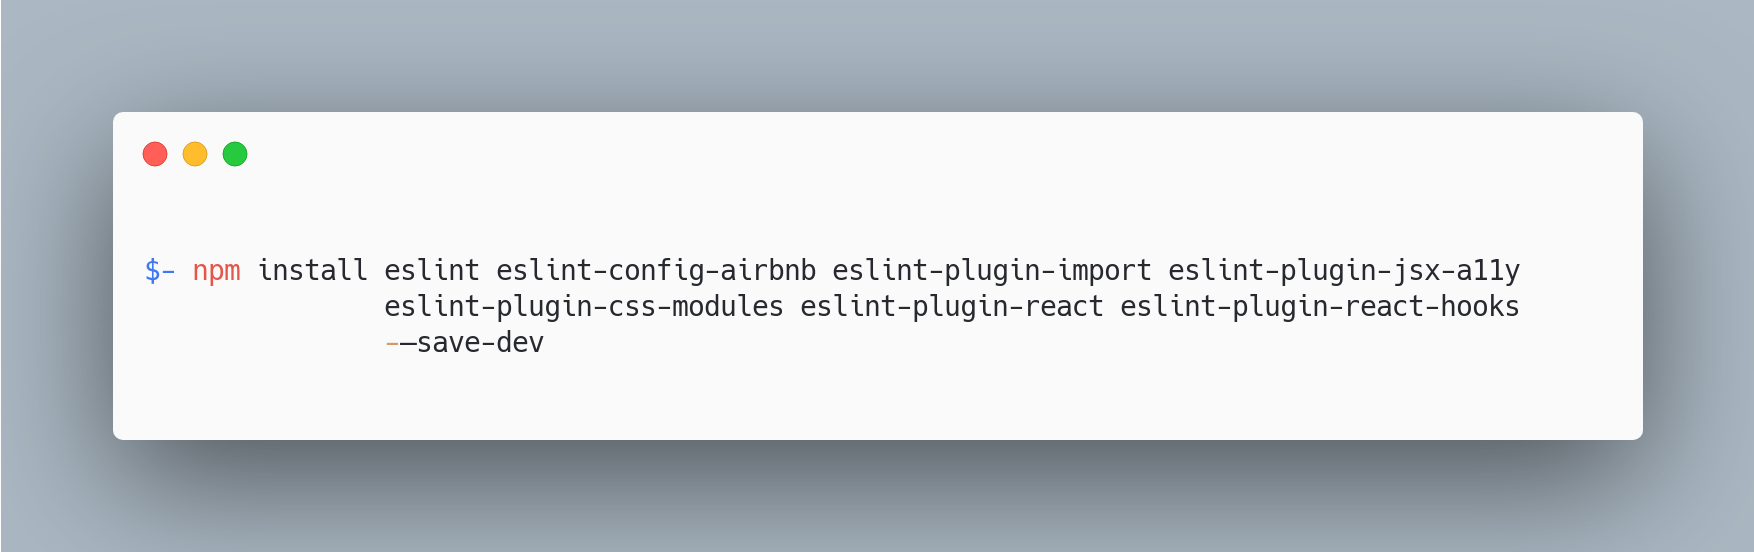
\includegraphics[width=1\textwidth]{./Imagenes/image14.png}
    \caption[Agregar ESLint]{Agregar ESLint}
    \end{figure}
    \newline
    \newline
    Dentro de las dependencias que agregamos se encuentran algunos complementos (plugins) que nos ayudan a dar formato a los archivos JSX, a verificar la sintaxis de React y  puede verificar que la importación de algún archivo realmente arroje un resultado.
    Debemos agregar un archivo en el que definiremos un conjunto de reglas específicas las cuales nuestros archivos van a cumplir, para agregar el archivo se debe ejecutar el siguiente comando.
    \newline
    \newline
     \begin{figure}[H]
    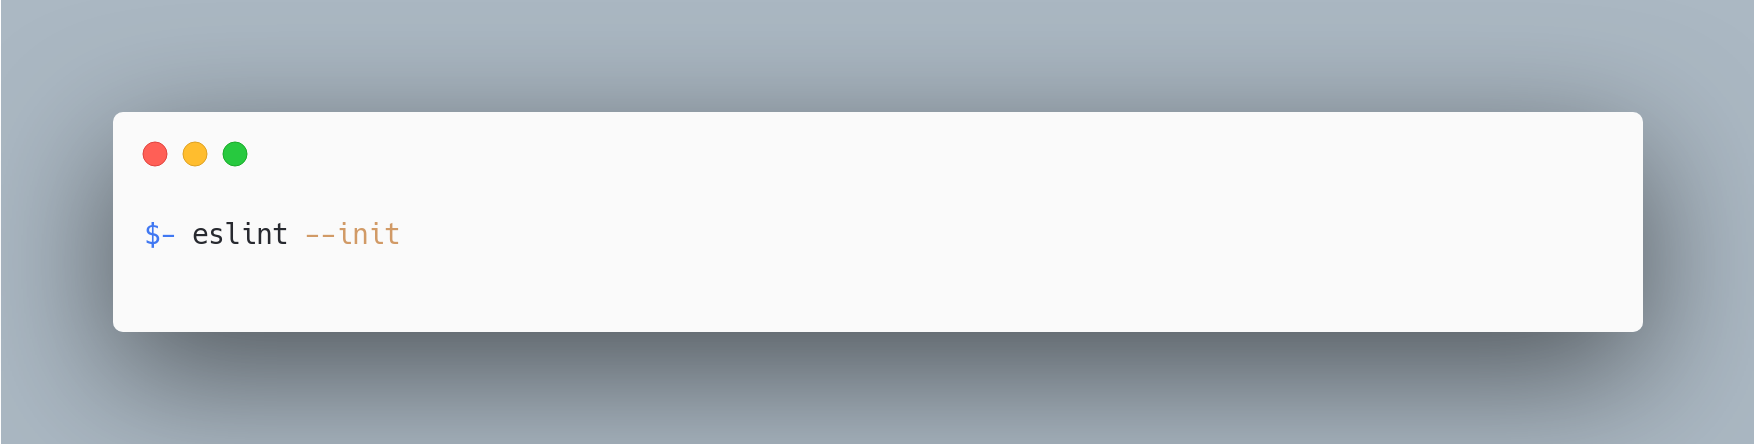
\includegraphics[width=1\textwidth]{./Imagenes/image32.png}
    \caption[Inicializar ESLint]{Inicializar ESLint}
    \end{figure}
    \newline
    \newline
    Después de ejecutar el comando este preguntara por datos para la configuración de ESLint, a continuación, se enlistan cada uno de los datos introducidos.
    \begin{itemize}
    \item \textbf{Uso de ESLint:  }Seleccionaremos el uso que le daremos a ESLint, que en este caso es checar sintaxis, encontrar problemas y forzar el estilo del código.
    \item \textbf{Tipo de módulos que usa el proyecto:} Seleccionaremos la opción JavaScript modules, por que es el tipo de importaciones y exportaciones que estaremos usando.
    \item \textbf{Framework por usar: }Seleccionaremos React.
    \item ¿Se usará TYPESCRIPT?: Se selecciona no. 
    \item ¿Donde se ejecutará?: Debemos seleccionar navegador.
    \item \textbf{Guía de estilos que se usará en el proyecto: } Nosotros elegiremos usar una guía popular  y después escogemos Airbnb.
    \item Formato del archivo de salida: Nosotros debemos escoger JavaScript.
    \end{itemize}
    Con esto tenemos todo listo para comenzar con el desarrollo de nuestra librería.
    \newpage
